
The estimation of vehicle motion parameters
utilizes smartphone built-in gyroscope and accelerometer.
It usually consists of two steps, coordinate alignment
and linear acceleration estimation.
Coordinate alignment refers to the process that transfers
the arbitrary coordinates of the smartphone to those of the car.  
Coordinate alignment provides us with the three-dimensional accelerometer
and gyroscope readings of the car \cite{wang2013sensing, hansenspeed}.
As illustrated in Fig. \ref{coordinates}, we use 
$[x, y, z]$ to represent the three dimensions of a smartphone
and use $[x', y', z']$ to represent the three dimensions
of a car. 
Coordinate alignment is the process that trains the rotation
matrix $R = [\hat{i}, \hat{j}, \hat{k}]$, 
where $\hat{i}$, $\hat{j}$ and $\hat{k}$ are three unit coordinate vectors,
so that $[x', y', z'] = [x, y, z] \times [\hat{i}, \hat{j}, \hat{k}]$.

\begin{figure}[!tbph]
	\begin{center}
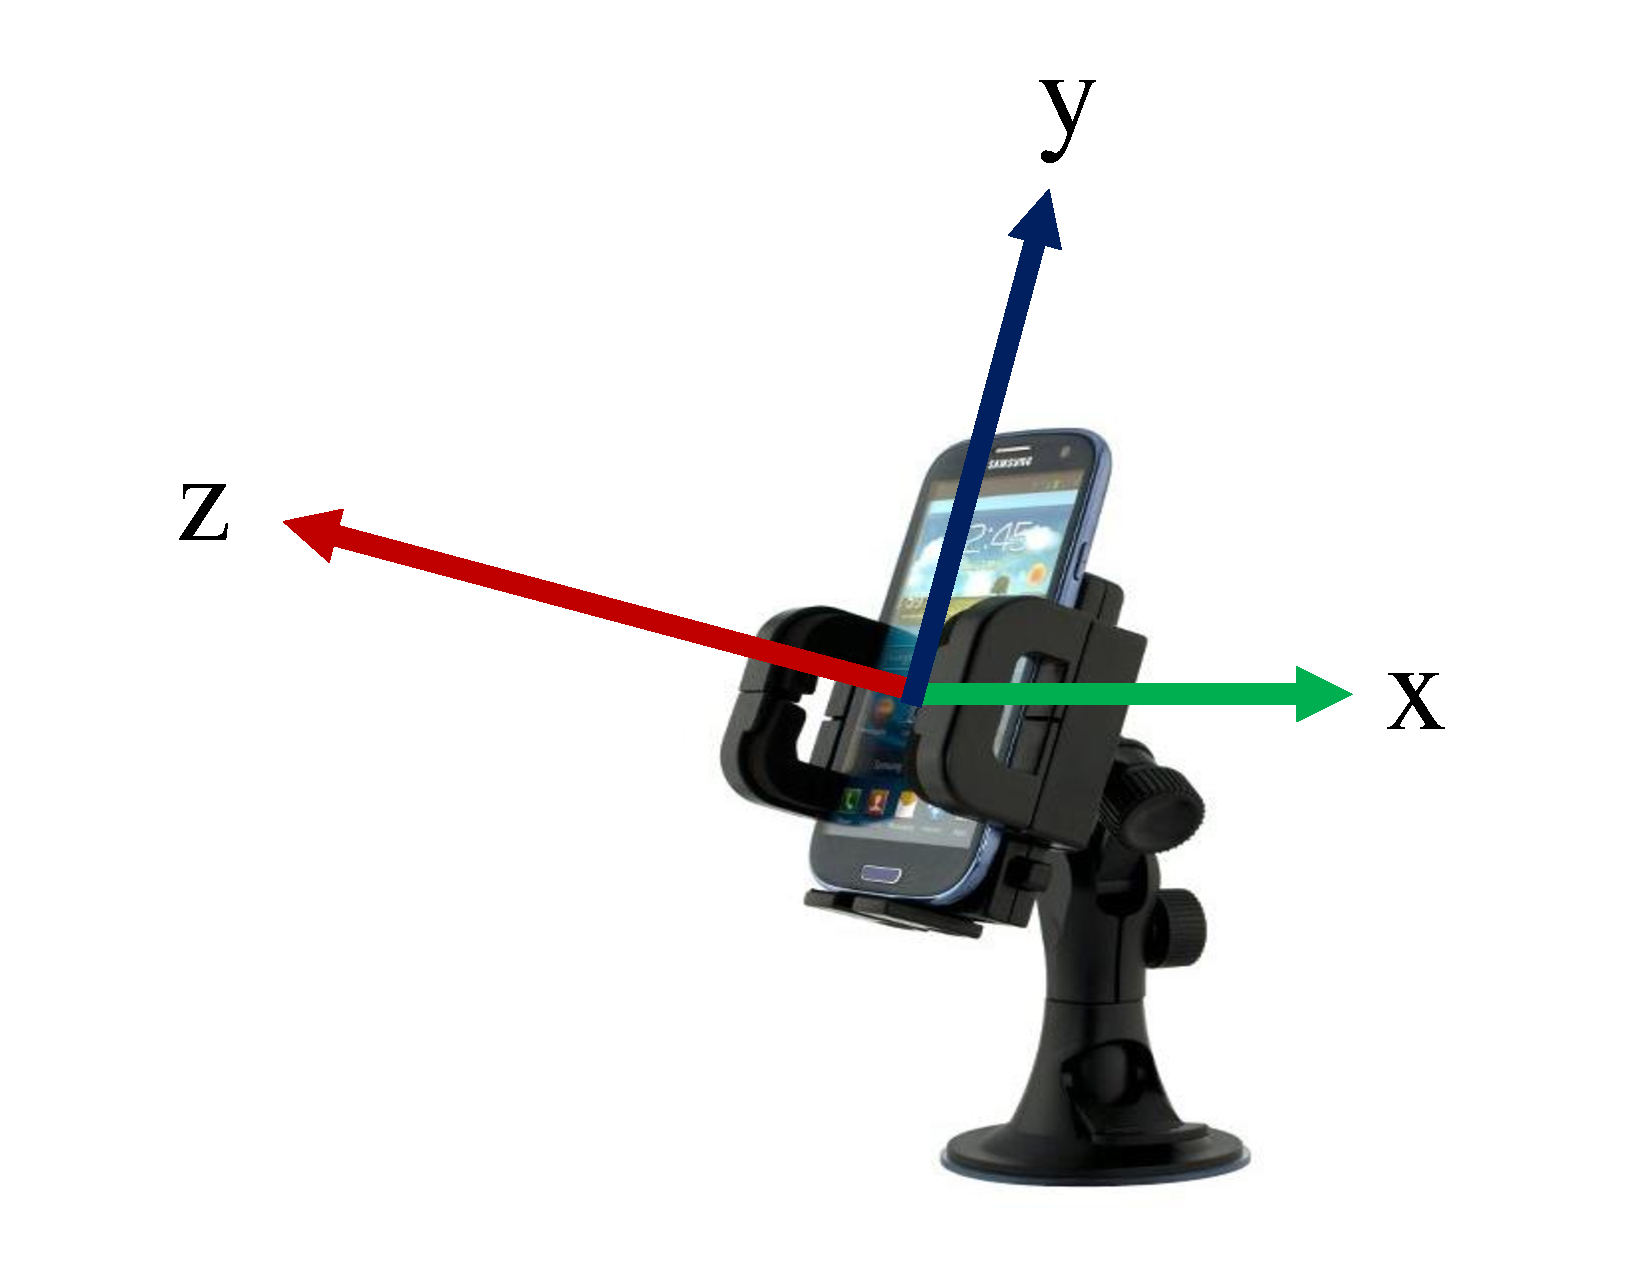
\includegraphics[width=2.4in,angle=0]{Figs/SlopeAware/phone3d.pdf}
\vspace{0.0cm}
\hspace{-1.0cm}
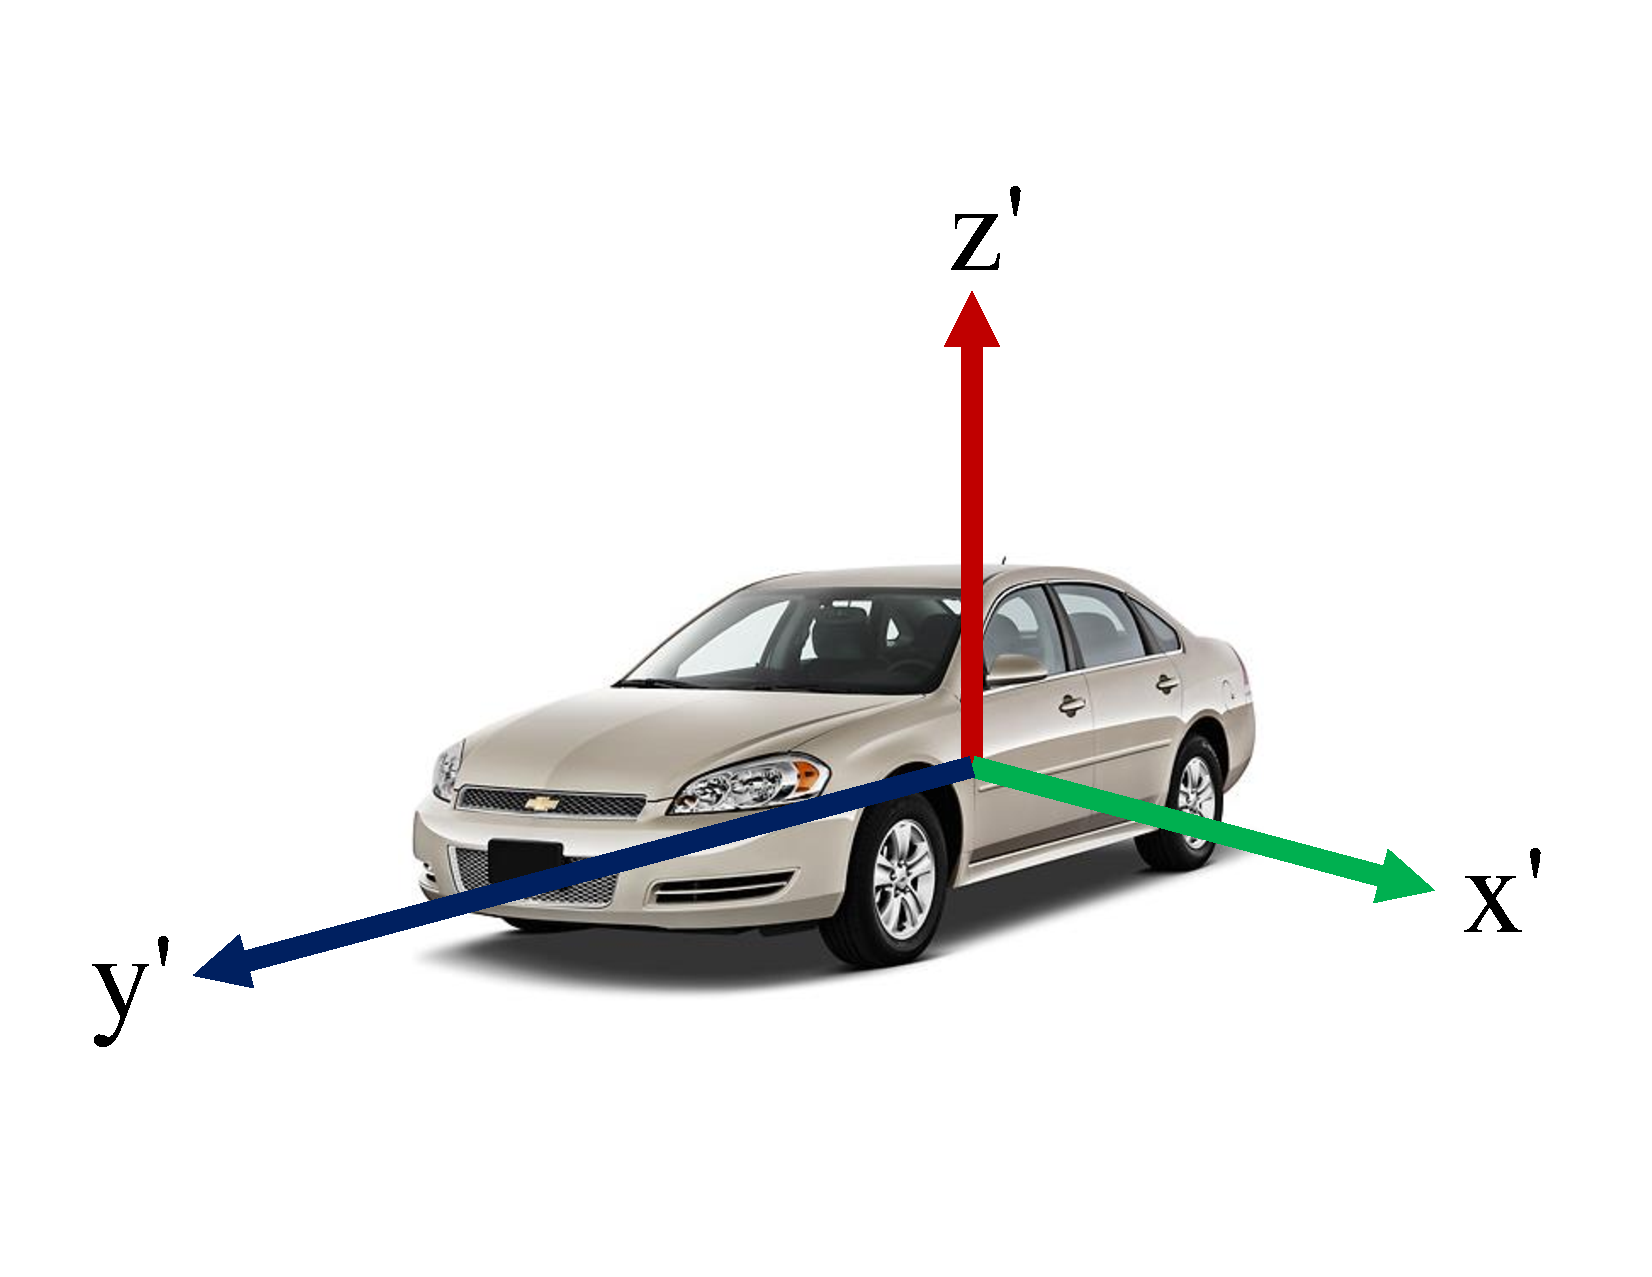
\includegraphics[width=2.4in,angle=0]{Figs/SlopeAware/car3d.pdf}
\vspace{-0.2cm}
\caption{Coordinate system difference between a smartphone $[x, y, z]$ and a car $[x', y', z']$.}
\vspace{0.2cm}
\label{coordinates}
\end{center}
\end{figure}



It should be noted that tracking the relative orientation 
(or coordinate alignment) is different from
and even more challenging than 
tracking the absolute orientation of 
a smartphone \cite{zhou2014use}. 
Tracking the absolute orientation of the phone is very useful for
many applications including walking direction
tracking \cite{roy2014smartphone}, 
3D road construction \cite{yang2015low}.
Estimating the relative orientation requires the algorithm
to track the heading direction of the car and estimate 
road slopes.
We will show that a road condition unaware algorithm
needs much more time to train the rotation matrix
between the smartphone and the car and causes 
false negatives/positives when capturing driving behaviors.
\subsection{State of the Art}

\begin{figure}[!tbph] \centering
    \begin{subfigure}[b]{\linewidth}    
    \begin{center}
	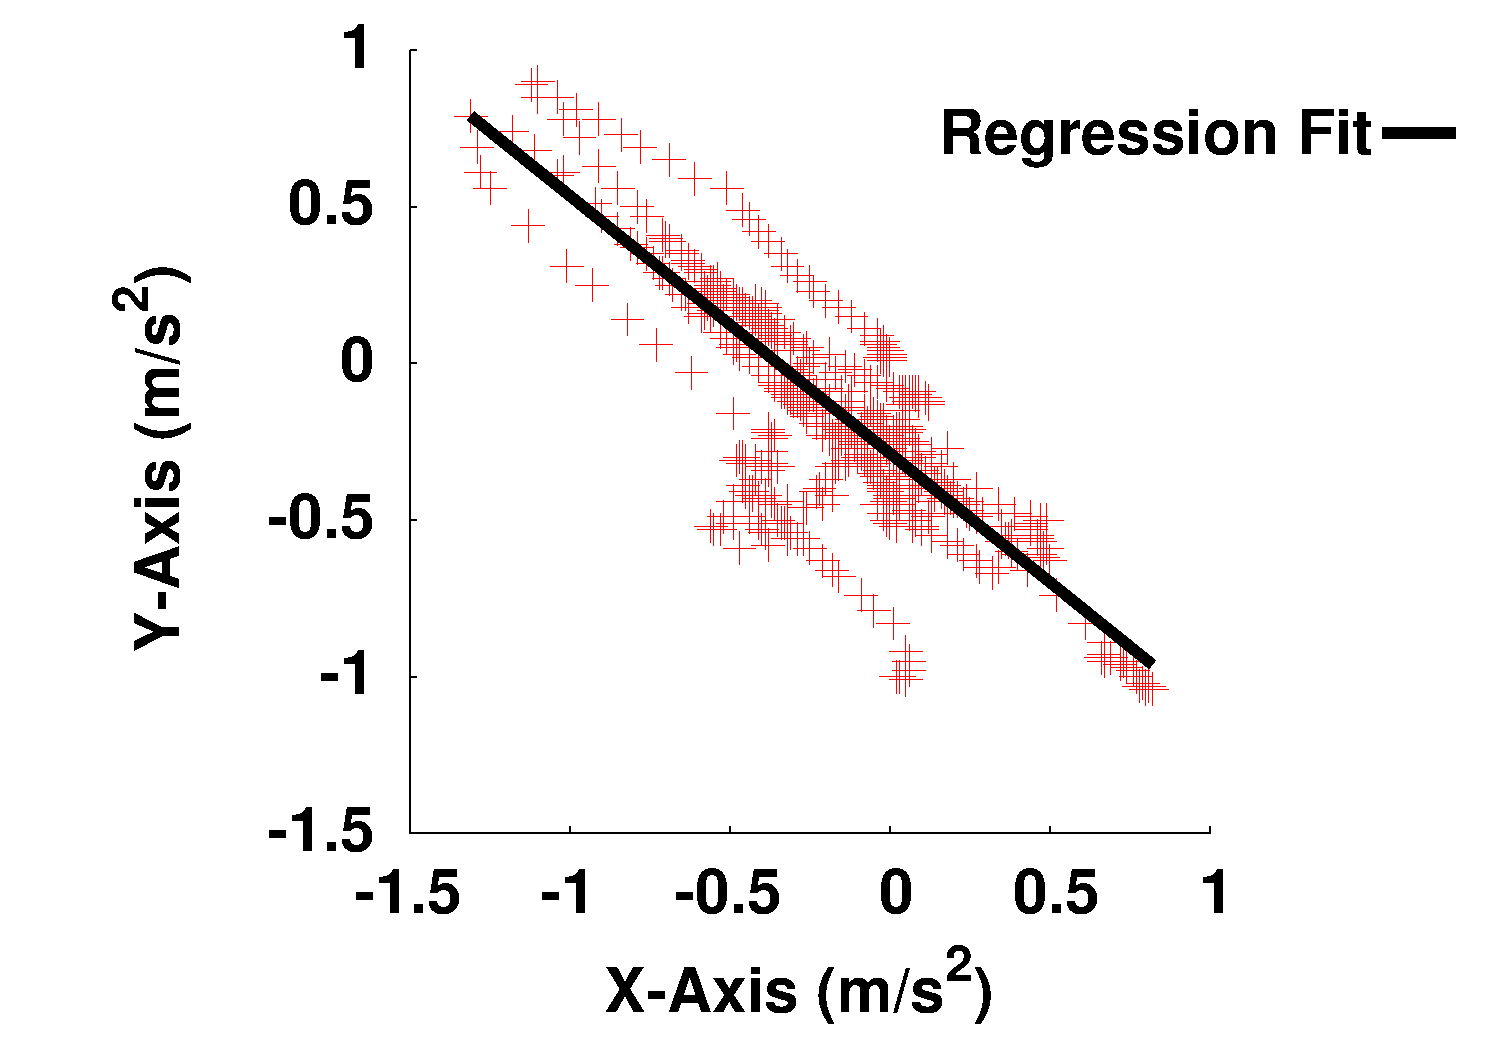
\includegraphics[width=3.2in,angle=0]{Figs/SlopeAware/stateoftheart.pdf}
        \caption{State of the Art}
        \label{direction:a}    
\end{center}
    \end{subfigure} 
    \begin{subfigure}[b]{\linewidth}
    \begin{center}
    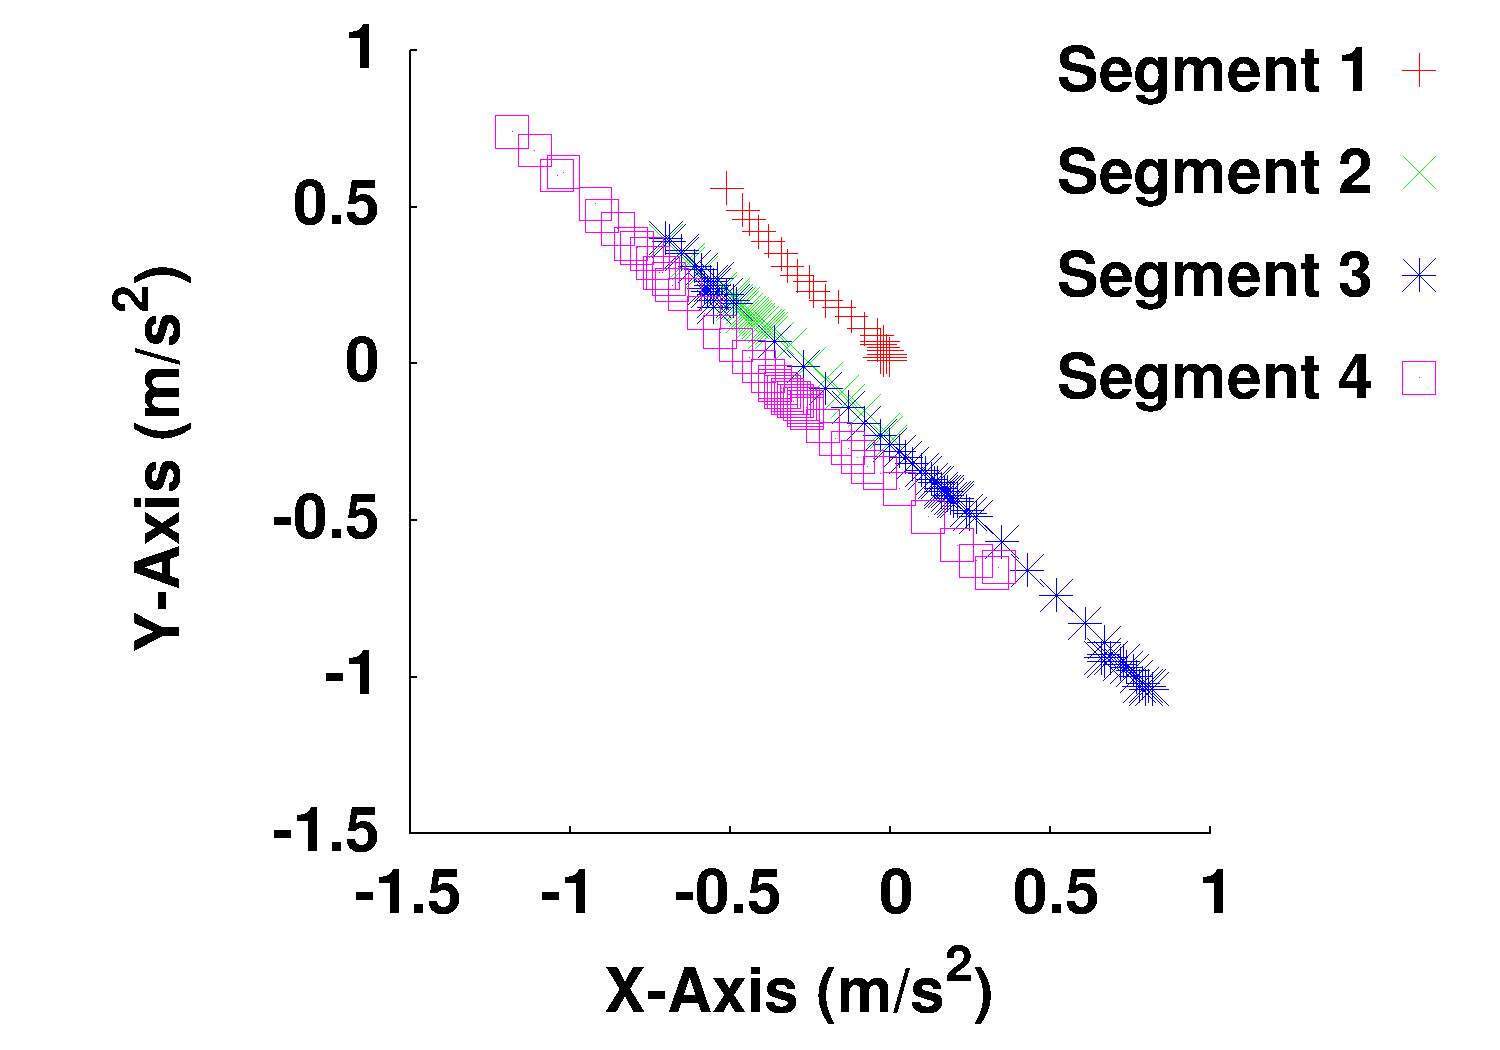
\includegraphics[width=3.2in,angle=0]{Figs/SlopeAware/direction.pdf}
         \caption{Selective training on the road segments, the four curves are extracted 
	 by accelerometer which are corresponding to the four training segments in Fig. \ref{training}.}
        \label{direction:b}
    \end{center}
    \end{subfigure} %
   \caption{Horizontal rotation matrix training, comparing 
  the state of the art (Fig. \ref{direction:a}) with selective training (Fig. \ref{direction:b}).}
\label{direction}
\vspace{-0.3cm}
\end{figure}



Coordinate alignment has been discussed in \cite{Mohan2008Nericell}, 
which relies on GPS to detect motions and straight line driving. 
A gyroscope has better accuracy for straight line driving detection
and low energy consumption than GPS,
so it is considered as a better alternative to GPS \cite{wang2013sensing}.
Coordinate alignment with gyroscope consists of three steps to derive the three 
unit coordinate vectors \cite{wang2013sensing}.
First, it obtains the constant components from these three accelerations
and derives the gravity acceleration. 
Second, it detects driving on straight roads and determines the 
heading direction of the car.
After the two out of three dimensions are determined, 
the last one can be derived from the right-hand rule.
Different from the absolute orientation estimation method proposed in \cite{zhou2014use}, 
coordinate alignment does not use magnetometer as 
the car body introduces continuous bias 
in magnetometer sensor readings \cite{wang2015determining}. 
Instead, it relies on sensor fusion of accelerometer and gyroscope \cite{wang2013sensing}. 




However, the solution in \cite{wang2013sensing} was designed for turn extraction
and not for capturing linear acceleration of the car driving in the context of sloping roads. 
It may cause misalignment and acceleration estimation errors 
due to two reasons.  
First, the constant components that are used to derive the gravity acceleration 
may be captured on a slope, which may cause the \emph{vertical misalignment} illustrated 
in Fig. \ref{slopecarphone}.
If the gravity accelerations are captured on a slope,
the accelerometer reading will show deceleration even when the car is stopped on a level road due to the gravitational effect.
The horizontal acceleration of a car will be underestimated or overestimated.
Second, determining the heading direction of a car requires 
lots of data points to fit the curve (or the direction), 
while the straight line driving may happen on slopes so different data points
from different slopes may not fit together (an illustration is shown in Fig. \ref{direction:a}).

\subsection{Slope-Aware Alignment}

We propose two techniques, selective training and slope gradient estimation at alignment time,
to resolve the issues of slope unaware coordinate alignment is not addressing.
When identifying the gravity accelerations, 
rather than capturing gravity accelerations at an arbitrary location, 
we propose to do it at the locations before and/or after 
the car is driving straight,
so that the data points collected in this road segment 
can be used to conduct slope gradient estimation.
When estimating the heading direction of a car, 
instead of putting all the training samples together, 
we propose to train the unit coordination vector separately 
with different road segments and refine the 
unit vector by combining the training results gradually.
  

\subsubsection{Selective Training}
\label{selectivetraining}
For easy understanding, we use the horizontal alignment (estimating
the heading direction of a car) as an example.
Vertical alignment is considered as a similar process.  
The process includes selecting the segments that the car is driving
straight, and estimating the intersection angle between the heading direction and the smartphone's horizontal coordinates. 
To derive the rotation matrix from discrete sensor data points, 
we need to fit the curve and find the direction unit vector. 
More data points can produce better accuracy. 
However, it is not the case when there are slopes 
make the lines of best fit deviate from the original point. 


Instead, we propose to use selective training that trains the horizontal
unit vector for each segment and combine each training results gradually with different weights.
The weight of each training segment is the function of the number of data points. 
The difference between these two approaches is shown in Fig. \ref{direction:a} and \ref{direction:b}. 
In Fig. \ref{direction:a}, we put all the data points when the car is driving 
straight (by using gyroscope) and fit the curve to expect a better
fitting accuracy. 
The slope of the curve is estimated to be $-0.84$. 
There are lots of straight driving segments as illustrated in Fig. \ref{training}, 
but not all of the segments are good for the training purpose. 
Each segment is selected based on the number of data points that
indicate the car is moving, 
as the entropy of the data points when the car is stopped is zero.   
In Fig. \ref{direction:b}, we separate four segments (also indicated 
in Fig. \ref{training}) and train the 
horizontal unit vector separately.
Clearly, this approach gives better view results that the four slopes of the 
fitting curves are $-0.98$, $-0.87$, $-0.93$ and $-0.95$, respectively. 
The weighted average is $-0.94$. 
The observation here is that each training segment gives better accuracy than
putting all the data points together and gradually training can improve the accuracy. 
Given the slope of the fitting curve or the rotation angle $\alpha$, 
we can derive the horizontal rotation matrix as

\[
R_h
	=
\begin{bmatrix}
   cos(\alpha) & -sin(\alpha) & 0 \\
   sin(\alpha) & cos(\alpha) & 0 \\
   0 & 0 & 1
\end{bmatrix}
\]



The indication of selective training is that slope-aware training enable 
faster and more accurate training results, so that a user
can have a better experience in a real-time application such as hard brake warning
(similar to snapshot \cite{snapshot} but infrastructure-free).


\subsubsection{Slope Gradient Estimation at Alignment Time}


\begin{figure}[!tbph]
\begin{center}
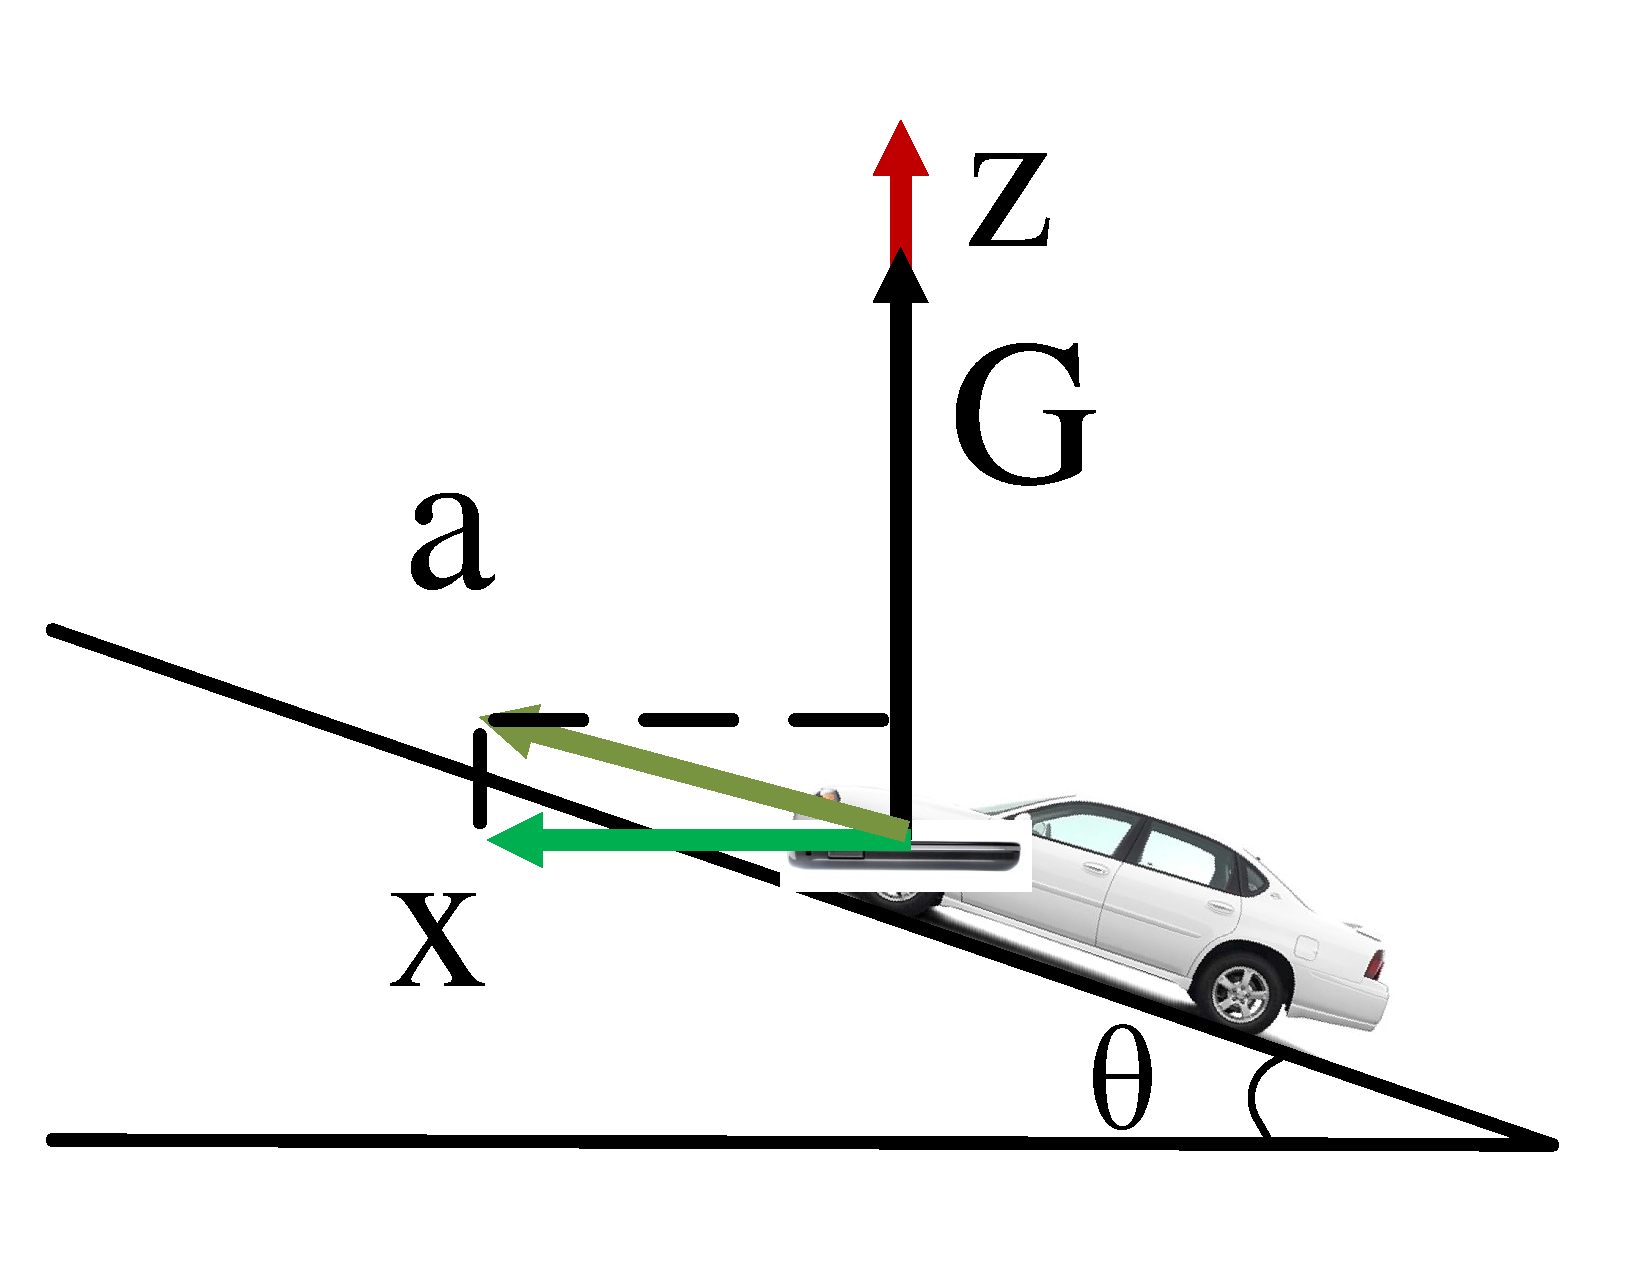
\includegraphics[width=2.0in, angle=0]{Figs/SlopeAware/slopeandcarphone.pdf}
\vspace{-0.0cm}
\caption{Slope gradient estimation at coordinate alignment time.}
\vspace{-0.3cm}
\label{slopecarphone}
\end{center}
\end{figure}

As discussed above, vertical misalignment causes acceleration estimation error due to the gravitational force. 
We estimate the slope of each segment to eliminate the vertical misalignment.
We use the same training segment to estimate the road slope gradient. 
First, we extract the gravity accelerations if a car stops on that road segment.
Then the road slope gradient can be trained in the same way as described in the previous section.



